% 西北农林科技大学科技类及IT类课程论文文档类(LaTeX模板)
\documentclass[
   projtype=report, % 实习类型,可选report(报告)或paper(论文),默认为report
   output=print,     % 输出类型,可选print(打印,不显示超链接颜色)
                   %           或epub(电子稿,显示超链接颜色),默认为epub
  ]{nwafuprojrep}

% 载入需要的宏包
\usepackage{floatrow}% 浮动体增强宏包
\usepackage{subcaption}% 子图排版
\usepackage{amsmath}% 数学宏包
\usepackage{booktabs}% 三线表格
\usepackage{longtable}% 跨页长表格
\usepackage{multirow,makecell}% 表格行合并,单元格处理
\usepackage{ulem}% 下划线
\usepackage[backend=biber,
                style=gb7714-2015,
                maxbibnames=99,% 著录所有作者
                maxcitenames=2,% 引用标注中最多显示2个作者
                mincitenames=1,% 3个及3个以上的作者截断为1个作者
                gbpub=false,
                gbnamefmt=familyahead,
                url=false,
                doi=false,
                isbn=false,
                gbfieldtype=true, % 输出学位论文标识
                ]{biblatex} % 参考文献

% =========命令行窗口及代码排版(自己开发的宏包)=========
% 请确保工作目录中存在boxie.sty、fvextra.sty和lstlinebgrd.sty三个文件
\usepackage{boxie}
% =========插图标注宏包(修改为标注框可以换行)=========
% 请确保工作目录中存在tikz-imglabels.sty文件
\usepackage{tikz-imglabels}
% =========流程图宏包(自己开发)=========
% 请确保工作目录中存在tikz-flowchart.sty文件
\usepackage{tikz-flowchart}

\usepackage{pgf-umlcd}% UML图宏包
\usepackage[ruled,linesnumbered]{algorithm2e}% 算法排版宏包
\usepackage{siunitx}% 标准单位符号宏包
\usepackage{csquotes}% 引号宏包
\usepackage{hyperref}% hyperref 需要最后引入

%%% Local Variables:
%%% mode: latex
%%% TeX-master:"../main.tex"
%%% End:

\usepackage{graphics}
\usepackage{float}
% 进行必要的设置
% ====================================================================================
% cquotes宏包的中文引号样式
% ====================================================================================
\DeclareQuoteStyle{zhquotestyle}% style name
    {\symbol{"201C}}% opening outer mark
    {\symbol{"201D}}% closing outer mark
    {\symbol{"2018}}% opening inner mark
    {\symbol{"2019}}% closing inner mark

\setquotestyle{zhquotestyle}

% ====================================================================================
% 改变表格字体
% ====================================================================================
\BeforeBeginEnvironment{tabular}{\small}%

% ====================================================================================
% 设置floatrow浮动体属性
% ====================================================================================
\DeclareFloatVCode{beforefig}{\vspace{-4pt}}
\DeclareFloatVCode{beforetab}{\vspace{-6pt}}
\DeclareFloatVCode{afterfloat}{\vspace{4pt}}
\floatsetup{postcode=afterfloat}
\floatsetup[table]{capposition=TOP, captionskip=2pt, objectset=centering, margins=centering, precode=beforetab}
\floatsetup[figure]{captionskip=4pt, objectset=centering, margins=centering, precode=beforefig}

% ====================================================================================
% 代码交叉引用命令\autoref的引用格式
% ====================================================================================
\def\cvcounterautorefname{代码}%
\renewcommand{\thecvcounter}{\arabic{cvcounter}}
\def\cvcounterautorefname~#1\null{代码~#1\null}%

%%% Local Variables:
%%% mode: latex
%%% TeX-master:"../main.tex"
%%% End:

% 专用术语宏命令
% ====================================================================================
% 西北农林科技大学各单位名称
% ====================================================================================
\newcommand{\nwafu}{西北农林科技大学}
\newcommand{\cie}{信息工程学院}

% ============自定义专有名词命令============
\newcommand{\cl}{\texttt{C}语言}
\newcommand{\ccpp}{\texttt{C/C++}}
\newcommand{\win}{\texttt{Windows}}
\newcommand{\ide}{\texttt{IDE}}
\newcommand{\gcc}{\texttt{GCC}}
\newcommand{\gpp}{\texttt{G++}}
\newcommand{\gnu}{\texttt{GNU}}
\newcommand{\cb}{\texttt{Code::Blocks}}
\newcommand{\mgww}{\texttt{MinGW}}
\newcommand{\mgw}{\texttt{MinGW32}}
\newcommand{\mgwww}{\texttt{MinGW-w64}}
\newcommand{\lumos}{\texttt{Linux}、\texttt{Unix}、\texttt{Mac OS}}
\newcommand{\unix}{\texttt{UNIX}}
\newcommand{\lnx}{\texttt{Linux}}
\newcommand{\mk}{\texttt{make}}
\newcommand{\ph}{\texttt{Path}}
\newcommand{\cmdd}{\texttt{cmd}}
\newcommand{\gdb}{\texttt{gdb}调试器}
\newcommand{\vside}{\texttt{Visual Studio}}
\newcommand{\mfile}{\texttt{Makefile}}
\newcommand{\tgt}{\texttt{target}}
\newcommand{\prqt}{\texttt{prerequisites}}
\newcommand{\cbv}{\texttt{17.12}}
\newcommand{\db}{\texttt{DEBUG}}
\newcommand{\dbger}{\texttt{Debugger}}
\newcommand{\cdb}{\texttt{cdb}调试器}
\newcommand{\gdbcmd}{\texttt{(gdb)}}
\newcommand{\bug}{\texttt{BUG}}
\newcommand{\ieee}{\texttt{IEEE754}标准}
\newcommand{\ascii}{\texttt{ASCII}}
\newcommand\vararg{变长形参列表}
\newcommand\varargfun{\vararg{}函数}
\newcommand{\cg}{\texttt{CGraph2D} 图形库}
\newcommand{\git}{分布式版本控制系统\texttt{Git}}
\newcommand{\github}{\texttt{Github}平台}
% ====================================


%%% Local Variables:
%%% mode: latex
%%% TeX-master:"../main.tex"
%%% End:

% 数学符号宏命令
% !TeX root = ./main.tex

% Adapted for use with ustcthesis.
% Original code is at https://github.com/goodfeli/dlbook_notation/blob/master/math_commands.tex

%%%%% NEW MATH DEFINITIONS %%%%%

\newcommand\ceil[1]{\lceil #1 \rceil}
\newcommand\floor[1]{\lfloor #1 \rfloor}


% Vectors
%\newcommand\Vector[1]{\symbf{#1}}

\newcommand\0{{\Vector{0}}}
\newcommand\vzero{{\Vector{0}}}
\newcommand\1{{\Vector{1}}}
\newcommand\vone{{\Vector{1}}}

\newcommand\va{{\Vector{a}}}
\newcommand\vb{{\Vector{b}}}
\newcommand\vc{{\Vector{c}}}
\newcommand\vd{{\Vector{d}}}
\newcommand\ve{{\Vector{e}}}
\newcommand\vf{{\Vector{f}}}
\newcommand\vg{{\Vector{g}}}
\newcommand\vh{{\Vector{h}}}
\newcommand\vi{{\Vector{i}}}
\newcommand\vj{{\Vector{j}}}
\newcommand\vk{{\Vector{k}}}
\newcommand\vl{{\Vector{l}}}
\newcommand\vm{{\Vector{m}}}
\newcommand\vn{{\Vector{n}}}
\newcommand\vo{{\Vector{o}}}
\newcommand\vp{{\Vector{p}}}
\newcommand\vq{{\Vector{q}}}
\newcommand\vr{{\Vector{r}}}
\newcommand\vs{{\Vector{s}}}
\newcommand\vt{{\Vector{t}}}
\newcommand\vu{{\Vector{u}}}
\newcommand\vv{{\Vector{v}}}
\newcommand\vw{{\Vector{w}}}
\newcommand\vx{{\Vector{x}}}
\newcommand\vy{{\Vector{y}}}
\newcommand\vz{{\Vector{z}}}

\newcommand\valpha{{\Vector{\alpha}}}
\newcommand\vbeta{{\Vector{\beta}}}
\newcommand\vgamma{{\Vector{\gamma}}}
\newcommand\vdelta{{\Vector{\delta}}}
\newcommand\vepsilon{{\Vector{\epsilon}}}
\newcommand\vtheta{{\Vector{\theta}}}
\newcommand\viota{{\Vector{\iota}}}
\newcommand\vkappa{{\Vector{\kappa}}}
\newcommand\vlambda{{\Vector{\lambda}}}
\newcommand\vmu{{\Vector{\mu}}}
\newcommand\vnu{{\Vector{\nu}}}
\newcommand\vxi{{\Vector{\xi}}}
\newcommand\vpi{{\Vector{\pi}}}
\newcommand\vrho{{\Vector{\rho}}}
\newcommand\vsigma{{\Vector{\sigma}}}
\newcommand\vtau{{\Vector{\tau}}}
\newcommand\vupsilon{{\Vector{\upsilon}}}
\newcommand\vphi{{\Vector{\phi}}}
\newcommand\vchi{{\Vector{\chi}}}
\newcommand\vpsi{{\Vector{\psi}}}
\newcommand\vomega{{\Vector{\omega}}}


% Matrix
\newcommand\MATRIX[1]{\symbf{#1}}

\newcommand\mA{{\MATRIX{A}}}
\newcommand\mB{{\MATRIX{B}}}
\newcommand\mC{{\MATRIX{C}}}
\newcommand\mD{{\MATRIX{D}}}
\newcommand\mE{{\MATRIX{E}}}
\newcommand\mF{{\MATRIX{F}}}
\newcommand\mG{{\MATRIX{G}}}
\newcommand\mH{{\MATRIX{H}}}
\newcommand\mI{{\MATRIX{I}}}
\newcommand\mJ{{\MATRIX{J}}}
\newcommand\mK{{\MATRIX{K}}}
\newcommand\mL{{\MATRIX{L}}}
\newcommand\mM{{\MATRIX{M}}}
\newcommand\mN{{\MATRIX{N}}}
\newcommand\mO{{\MATRIX{O}}}
\newcommand\mP{{\MATRIX{P}}}
\newcommand\mQ{{\MATRIX{Q}}}
\newcommand\mR{{\MATRIX{R}}}
\newcommand\mS{{\MATRIX{S}}}
\newcommand\mT{{\MATRIX{T}}}
\newcommand\mU{{\MATRIX{U}}}
\newcommand\mV{{\MATRIX{V}}}
\newcommand\mW{{\MATRIX{W}}}
\newcommand\mX{{\MATRIX{X}}}
\newcommand\mY{{\MATRIX{Y}}}
\newcommand\mZ{{\MATRIX{Z}}}

\newcommand\mGamma{{\MATRIX{\Gamma}}}
\newcommand\mDelta{{\MATRIX{\Delta}}}
\newcommand\mTheta{{\MATRIX{\Theta}}}
\newcommand\mLambda{{\MATRIX{\Lambda}}}
\newcommand\mXi{{\MATRIX{\Xi}}}
\newcommand\mPi{{\MATRIX{\Pi}}}
\newcommand\mSigma{{\MATRIX{\Sigma}}}
\newcommand\mUpsilon{{\MATRIX{\Upsilon}}}
\newcommand\mPhi{{\MATRIX{\Phi}}}
\newcommand\mPsi{{\MATRIX{\Psi}}}
\newcommand\mOmega{{\MATRIX{\Omega}}}


% Tensor
\newcommand\tens[1]{\symbfsf{#1}}
\newcommand\tA{{\tens{A}}}
\newcommand\tB{{\tens{B}}}
\newcommand\tC{{\tens{C}}}
\newcommand\tD{{\tens{D}}}
\newcommand\tE{{\tens{E}}}
\newcommand\tF{{\tens{F}}}
\newcommand\tG{{\tens{G}}}
\newcommand\tH{{\tens{H}}}
\newcommand\tI{{\tens{I}}}
\newcommand\tJ{{\tens{J}}}
\newcommand\tK{{\tens{K}}}
\newcommand\tL{{\tens{L}}}
\newcommand\tM{{\tens{M}}}
\newcommand\tN{{\tens{N}}}
\newcommand\tO{{\tens{O}}}
\newcommand\tP{{\tens{P}}}
\newcommand\tQ{{\tens{Q}}}
\newcommand\tR{{\tens{R}}}
\newcommand\tS{{\tens{S}}}
\newcommand\tT{{\tens{T}}}
\newcommand\tU{{\tens{U}}}
\newcommand\tV{{\tens{V}}}
\newcommand\tW{{\tens{W}}}
\newcommand\tX{{\tens{X}}}
\newcommand\tY{{\tens{Y}}}
\newcommand\tZ{{\tens{Z}}}


% Graph
\newcommand\gA{{\mathcal{A}}}
\newcommand\gB{{\mathcal{B}}}
\newcommand\gC{{\mathcal{C}}}
\newcommand\gD{{\mathcal{D}}}
\newcommand\gE{{\mathcal{E}}}
\newcommand\gF{{\mathcal{F}}}
\newcommand\gG{{\mathcal{G}}}
\newcommand\gH{{\mathcal{H}}}
\newcommand\gI{{\mathcal{I}}}
\newcommand\gJ{{\mathcal{J}}}
\newcommand\gK{{\mathcal{K}}}
\newcommand\gL{{\mathcal{L}}}
\newcommand\gM{{\mathcal{M}}}
\newcommand\gN{{\mathcal{N}}}
\newcommand\gO{{\mathcal{O}}}
\newcommand\gP{{\mathcal{P}}}
\newcommand\gQ{{\mathcal{Q}}}
\newcommand\gR{{\mathcal{R}}}
\newcommand\gS{{\mathcal{S}}}
\newcommand\gT{{\mathcal{T}}}
\newcommand\gU{{\mathcal{U}}}
\newcommand\gV{{\mathcal{V}}}
\newcommand\gW{{\mathcal{W}}}
\newcommand\gX{{\mathcal{X}}}
\newcommand\gY{{\mathcal{Y}}}
\newcommand\gZ{{\mathcal{Z}}}


% Sets
\newcommand\sA{{\mathbb{A}}}
\newcommand\sB{{\mathbb{B}}}
\newcommand\sC{{\mathbb{C}}}
\newcommand\sD{{\mathbb{D}}}
% Don't use a set called E, because this would be the same as our symbol
% for expectation.
\newcommand\sF{{\mathbb{F}}}
\newcommand\sG{{\mathbb{G}}}
\newcommand\sH{{\mathbb{H}}}
\newcommand\sI{{\mathbb{I}}}
\newcommand\sJ{{\mathbb{J}}}
\newcommand\sK{{\mathbb{K}}}
\newcommand\sL{{\mathbb{L}}}
\newcommand\sM{{\mathbb{M}}}
\newcommand\sN{{\mathbb{N}}}
\newcommand\sO{{\mathbb{O}}}
\newcommand\sP{{\mathbb{P}}}
\newcommand\sQ{{\mathbb{Q}}}
\newcommand\sR{{\mathbb{R}}}
\newcommand\sS{{\mathbb{S}}}
\newcommand\sT{{\mathbb{T}}}
\newcommand\sU{{\mathbb{U}}}
\newcommand\sV{{\mathbb{V}}}
\newcommand\sW{{\mathbb{W}}}
\newcommand\sX{{\mathbb{X}}}
\newcommand\sY{{\mathbb{Y}}}
\newcommand\sZ{{\mathbb{Z}}}


% Random variables
\newcommand\RandomVariable[1]{\symit{#1}}

\newcommand\rA{{\RandomVariable{A}}}
\newcommand\rB{{\RandomVariable{B}}}
\newcommand\rC{{\RandomVariable{C}}}
\newcommand\rD{{\RandomVariable{D}}}
\newcommand\rE{{\RandomVariable{E}}}
\newcommand\rF{{\RandomVariable{F}}}
\newcommand\rG{{\RandomVariable{G}}}
\newcommand\rH{{\RandomVariable{H}}}
\newcommand\rI{{\RandomVariable{I}}}
\newcommand\rJ{{\RandomVariable{J}}}
\newcommand\rK{{\RandomVariable{K}}}
\newcommand\rL{{\RandomVariable{L}}}
\newcommand\rM{{\RandomVariable{M}}}
\newcommand\rN{{\RandomVariable{N}}}
\newcommand\rO{{\RandomVariable{O}}}
\newcommand\rP{{\RandomVariable{P}}}
\newcommand\rQ{{\RandomVariable{Q}}}
\newcommand\rR{{\RandomVariable{R}}}
\newcommand\rS{{\RandomVariable{S}}}
\newcommand\rT{{\RandomVariable{T}}}
\newcommand\rU{{\RandomVariable{U}}}
\newcommand\rV{{\RandomVariable{V}}}
\newcommand\rW{{\RandomVariable{W}}}
\newcommand\rX{{\RandomVariable{X}}}
\newcommand\rY{{\RandomVariable{Y}}}
\newcommand\rZ{{\RandomVariable{Z}}}

% Random vectors
\newcommand\RandomVector[1]{\symbf{#1}}

\newcommand\rvA{{\RandomVector{A}}}
\newcommand\rvB{{\RandomVector{B}}}
\newcommand\rvC{{\RandomVector{C}}}
\newcommand\rvD{{\RandomVector{D}}}
\newcommand\rvE{{\RandomVector{E}}}
\newcommand\rvF{{\RandomVector{F}}}
\newcommand\rvG{{\RandomVector{G}}}
\newcommand\rvH{{\RandomVector{H}}}
\newcommand\rvI{{\RandomVector{I}}}
\newcommand\rvJ{{\RandomVector{J}}}
\newcommand\rvK{{\RandomVector{K}}}
\newcommand\rvL{{\RandomVector{L}}}
\newcommand\rvM{{\RandomVector{M}}}
\newcommand\rvN{{\RandomVector{N}}}
\newcommand\rvO{{\RandomVector{O}}}
\newcommand\rvP{{\RandomVector{P}}}
\newcommand\rvQ{{\RandomVector{Q}}}
\newcommand\rvR{{\RandomVector{R}}}
\newcommand\rvS{{\RandomVector{S}}}
\newcommand\rvT{{\RandomVector{T}}}
\newcommand\rvU{{\RandomVector{U}}}
\newcommand\rvV{{\RandomVector{V}}}
\newcommand\rvW{{\RandomVector{W}}}
\newcommand\rvX{{\RandomVector{X}}}
\newcommand\rvY{{\RandomVector{Y}}}
\newcommand\rvZ{{\RandomVector{Z}}}

\newcommand\laplace{\mathrm{Laplace}} % Laplace distribution

\newcommand\E{\mathbb{E}}
\newcommand\Ls{\mathcal{L}}
\newcommand\R{\mathbb{R}}
\newcommand\emp{\tilde{p}}
\newcommand\lr{\alpha}
\newcommand\reg{\lambda}
\newcommand\rect{\mathrm{rectifier}}
\newcommand\softmax{\mathrm{softmax}}
\newcommand\sigmoid{\sigma}
\newcommand\softplus{\zeta}
\newcommand\KL{D_{\mathrm{KL}}}
\newcommand\Var{\mathrm{Var}}
\newcommand\standarderror{\mathrm{SE}}
\newcommand\Cov{\mathrm{Cov}}
% Wolfram Mathworld says $L^2$ is for function spaces and $\ell^2$ is for vectors
% But then they seem to use $L^2$ for vectors throughout the site, and so does
% wikipedia.
\newcommand\normlzero{L^0}
\newcommand\normlone{L^1}
\newcommand\normltwo{L^2}
\newcommand\normlp{L^p}
\newcommand\normmax{L^\infty}

\DeclareMathOperator*{\argmax}{arg\,max}
\DeclareMathOperator*{\argmin}{arg\,min}

\DeclareMathOperator{\sign}{sign}
\DeclareMathOperator{\Tr}{Tr}
\let\ab\allowbreak


% 设置封面基本信息,\linebreak 前面不要有空格,
% 中文之间的空格无法消除
% 另,在\nwafuset中不可以出现空行
\nwafuset{
  college = {信息工程学院},            % 学院名称
  projname = {面向对象程序设计},       % 实践课程名称
  title = {超市进销管理系统设计与实现},  % 实习报告题目
  stuno = {2019013121},              % 学号
  author = {林炅},             % 姓名
  major = {计算机科学与技术},          % 专业
  classid = {1903},                   % 班级(只填写数字,不要有其它内容)
  adviser = {王泽鹏},                   % 指导教师姓名
  startdate = {2020年8月24日},        % 实践起始日期
  enddate = {9月5日},        % 实践结束日期
}

\begin{document} %在document环境中撰写文档

%%%%%%%%%%%%%%%%%%%%%%%%%%%%%%%%%%%%%%%%
% 封面及目录,无需改动此处代码
% 面页,需要在导言区用\nwafuset命令填写基本信息
\makecover
\tableofcontents
\newpage
\cleardoublepage
\section{综合训练目的与要求}
\subsection{目的}
\begin{enumerate}
	\item 
	通过一学期对于面向对象程序课程的学习,理解面向对象程序设计的思想,了解面向对象程序设计的几大特点,抽象性,封装性,继承性,和多态性。并运用所学的思想,进行软件的开发实现,并能够完成解决一些实际问题
	\item 
	通过团队协作,采用面向对象程序设计的思想(类的设计,抽象,封装,包含与继承,多态性,UML图)进行项目开发。
	\item 
	通过\ccpp 编程,面向对象分析与设计,增加软件的健壮性,使程序的重用性、可维护性等等更强。结合Qt 中的一些类,进行界面上的设计,充分利用Qt 信号与槽的机制实现界面与槽函数直接的链接,实现界面与类之间的使用。
\end{enumerate}
\subsection{要求}
	采用面向对象程序设计思想设计Good 类,并在类中申请商店的各个私有属性,并设计成员函数用于调取和设置类中的私有成员。基于Good 类,实现超市进销管理系统。通过将商品名称与Good *关联,实现在系统中完成对超市商品数据信息的新增、删除、查找、修改等等操作,并实现打印库存,打印当日流水清单,打印购物清单等等操作.

\section{综合训练任务}
\subsection{综合任务}
\begin{enumerate}
	\item 采用面向对象程序设计思想设计Good 类,并在类中申请商店的各个私有属性,并设计成员函数用于调取和设置类中的私有成员。基于Good 类,实现超市进销管理系统.
	\item 实现登录界面,对输入正确用户名及密码的用户实行通过进入超市进销管理系统。
	\item 通过QMap 完成对超市进销系统商品的管理,实现能够新增商品,并对其进行保存。
	\item 实现对超市库存中的商品进行库存商品管理,实现对库存的展示,对库存中商品的查找,删除,修改,以及反馈库存中缺货商品名称。
	\item 实现超市销售管理,记录并保存一天的流水清单,并能够计算当日的营业额。
	\item 实现用户购买界面,允许用户将商品加入购物车,并完成结算,打印小票购物清单操作
\end{enumerate}
\subsection{个人任务}
\begin{enumerate}
	\item 通过与队友讨论,两人一起通过功能与需求的分析得到软件基本上所需要的功能和界面的大致布局设计,并以此作为参考,辅助队友进行主界面的搭建。
	\item 采用面向对象思想设计,运用STL库中的QMap 键值对用于存储商品信息Good*,以便于管理商品库存。
	\item 设计槽函数,负责与队友设计的ui界面连接,用QMap 的功能实现键值对的查询,删除,新增,查找功能,以及对商品流水情况和收入情况进行输出。
	\item 设计文件处理系统,实现能够对库存商品总信息,购物清单信息,当日流水清单的保存。
	\item 设计登录界面,将登录界面QWidget 与QMainWindow 主界面进行连接,实现登录完成后跳转至主界面。 
\end{enumerate}
\section{总体设计}
主要模块分为四块:
\begin{enumerate}
	\item 文件处理模块:主要负责文件的写入,以及界面上相应文件功能的实现(保存),分别完成对用户购物清单,库存商品信息,和当日流水情况的打印保存。
	\item 价格计算模块:用槽函数与QPushButton 连接实现能够计算出超市当日营业额计算以及每个用户购物车商品的价格计算。
	\item 商品管理模块:完成新增商品,删除商品,修改商品,查找商品。
	\item 商品信息展示模块:展示库存商品信息,展示本次商品进销信息,展示用户购物车商品信息。
\end{enumerate}
\begin{figure}[htbp]
% 允许各个位置
\centering
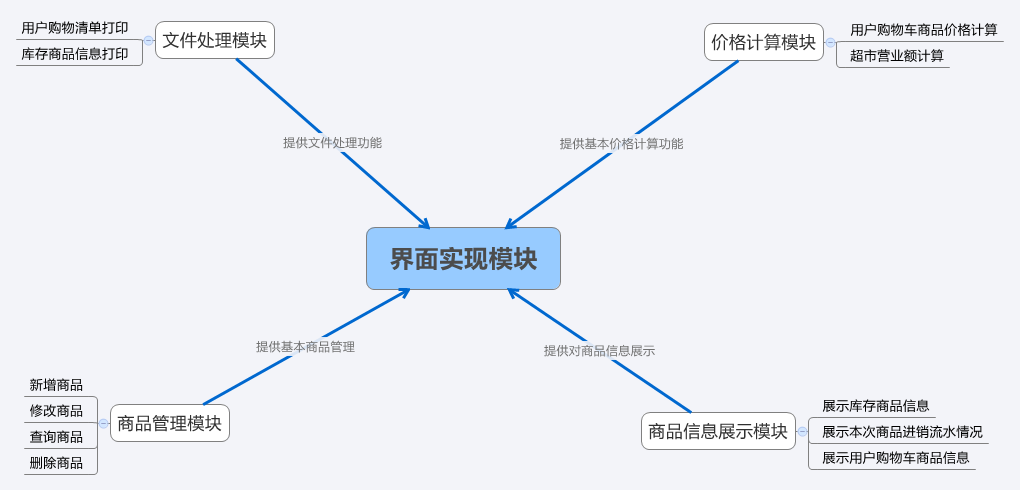
\includegraphics[width=1.0\textwidth]{界面实现模块.png}
\caption[模块设计]{模块设计图}\label{fig-jiemian}
\end{figure}
负责的模块:
\begin{enumerate}
	\item 商品的库存管理功能的设计和实现,通过STL库中的QMap 来实现对库存中的 商品的查看,查找,修改以及删除
	\item 商品的销售管理功能的设计和实现,通过对新增商品和卖出商品时的操作进行保存记录,并查看当日超市营业的总收入
	\item 超市的登录界面的设计和连接,设计登录界面,并将其与MainWindow 主窗口进行连接,输入正确后转入主窗口。
	\item 用户购物清单,库存商品信息以及超市进销库存流水情况打印的功能的实现。
\end{enumerate}
\subsubsection{商品的库存管理功能的设计和实现}
对商品的库存管理,我分为了QMenu菜单栏中的一个库存管理选项,在其子类的QAction中,我们增加了库存查看和信息修改两个功能。这个功能的设定,就是为了方便完成对在库存中的商品信息的管理,能够实时查看当前商品的内容,以及对这些内容进行修改。

总体的设计思路为,运用QMap的成员函数QMap.find、QMap.erase、QMap.value实现查询QMap内容,删除键值对,获取商品数据,通过与LineEdit结合,通过按钮连接槽函数实现,完成对商品数据的管理。运用QMap的迭代器,实现对QMap的遍历,并逐个在QTableView中输出展示。同时,为了防止出现缺货现象,在我们的超市进销管理系统中,新增了一个缺货查询功能,当使用QMap中的查询功能,查询到某件商品的数量减为0时,系统提示该商品已经缺货,建议补货操作。

\subsubsection{商品的销售管理功能的设计和实现}
对于超市的销售管理功能,我分为了QMenu菜单栏中的一个销售管理选项,在其子类的QAction中,新增加账目功能。功能的设定,方便用户能够查看到超市库存的进销情况,能够看到进货,卖货的各项数据。以及对商品总计的购物价格的统计总和,计算出营业总额。

总体实现的设计思路如下,库存进销情况展示分为了入库展示和出库展示,分别在入库时,将入库信息打印到本界面的QTextEdit 中,同理在购物车点击结算后,输出出库商品以及其信息到本界面的QTextEdit 中。这样的操作需要创建一个全局变量,在两个不同的槽函数中保存库存的进销情况。
\subsubsection{超市的登录界面的设计和连接}
对于超市的登录界面功能的实现,在界面中创建了用户名与密码以及对应的输入框QTextEdit,分别再创建关闭和登陆两个按钮完成界面的设计。修改一些界面QTextEdit的属性,使之更加符合真实登录环境。

界面的总体的实现和连接如下,创建的是一个新的ui界面,并在界面中放入想要的组件,并将按钮与槽函数连接,点击关闭按钮时,槽函数使创建的ui窗口界面关闭。点击登录便判断条形框中输入是否与程序预设的用户名和密码是否相同。相同则关闭当前登录界面弹出登录成功提醒并且打开主窗口,否则要清空QTextEdit,并报出失败登录提示,等待重新输入直到正确。
\subsubsection{文件处理打印功能的设计与实现}
对于文件处理打印功能的设计,我们分别使用在了三个方面,对库存管理中的库存商品情况的清单打印,对销售管理的商品进销情况的清单打印,以及对结算界面的所购买的商品进行清单打印

文件处理打印功能的总体实现情况如下,使用QT中的QFileDialog类来完成点击按钮跳出另存为界面,用其中的getSaveFileName(this,”保存”,QDir::currentPath(),”文本文件(*.txt)”);成员函数实现特定保存文件位置,调出设置文件文本框,期间还要判断存放的商品名字不能为空。接下来,使用QFile来保存文本框中的内容至所规定的文件中,创建文本输出流QTextStream ,分别调取库存管理中的库存商品情况 、销售管理的商品进销情况以及结算界面的所购买的商品购物车至所创建的输出流中。由于回车指令有些不同,需要在文本中做些替换操作。结束读入后,关闭文件清除QFile,释放内存,提示输出成功即可。
\section{详细设计说明}
Qt界面的设计与实现模块的详细说明:
\subsection{第一个部分:商品库存管理功能的设计和实现}
通过对项目的需求分析,然后通过进一步的功能的调整与确认,分析出所需要的功能为:库存查看,和信息修改,其中商品信息修改中包含对给定商品的查找,修改以及删除。在队友实现的商品入库后,完成对QMap中所保存的内容进行各种操作。
\subsubsection{信息修改}
信息修改中包括对给定的商品名称,用QMap中的find函数查询到商品的所有保存信息,并可以选择对已保存的商品信息展示在lineedit 中进行修改,并确认修改,或者直接在QMap 中删除该项商品所存在信息。
分别使用map.find、map.erase以及直接对map对应点Good*类中的成员用set进行修改
具体实现如下:代码清单\ref{code1}、\ref {code2}、\ref{code3}

\begin{langCVOne}[C++][code1][QT]{查询代码}
void MainWindow::on_findbtn_2_clicked()
{
  if(shop.find(ui->goodname_2->text())!=shop.end())
  {
      ui->barcode_2->setText(shop.find(ui->goodname_2->text()).value()->getcode());
      ui->amount_2->setText(number);
      ui->inprice->setText(inprice);
      ui->outprice->setText(outprice);
      ui->sup_2->setText(shop.find(ui->goodname_2->text()).value()->getsupplier());
      QMessageBox::information(this,"查询提示","已为你查询到商品全部信息");
  }
  else
  {
      QMessageBox::information(this,"查询提示","库存中没有该商品");
  }
}
\end{langCVOne}
\begin{langCVOne}[C++][code2][QT]{删除代码}
void MainWindow::on_deletebtn_clicked()
{
    shop.erase(shop.find(ui->goodname_2->text()));
    ui->goodname_2->clear();
    ui->barcode_2->clear();
    ui->amount_2->clear();
    ui->inprice->clear();
    ui->outprice->clear();
    ui->sup_2->clear();
    QMessageBox::information(this,"修改提示",ui->goodname_2->text()+"商品已被删除");
}
\end{langCVOne}
\begin{langCVOne}[C++][code3][QT]{修改代码}
void MainWindow::on_changebtn_clicked()
{
    shop[ui->goodname_2->text()]->setcode(ui->barcode_2->text());
    shop[ui->goodname_2->text()]->setnumber(ui->amount_2->text().toInt());
    shop[ui->goodname_2->text()]->setinprice(ui->inprice->text().toDouble());
    shop[ui->goodname_2->text()]->setoutprice(ui->outprice->text().toDouble());
    shop[ui->goodname_2->text()]->setsupplier(ui->sup_2->text());
    QMessageBox::information(this,"修改提示",ui->goodname_2->text()+"商品信息已经修改");
}
\end{langCVOne}
\subsubsection{库存查看}
库存查看允许用户查看目前在QMap 中保存的所有商品信息,用迭代器it遍历QMap 便能得到全部商品信息输出,呈现商品信息使用的QT部件QTableView 以表格形式呈现。并当某件商品数量为0时,输出展示当前缺货商品,方便管理员进货。


创建TableView 表格,在头文件创建QTableView *表格视角和 QStandardItemModel *标准模型项指针。并声明inittable函数用于生成连接表格。在函数中,添加表头,准备数据模型,利用setModel()方法将数据模型与QTableView绑定。随后修改表格的部分属性以满足产品需求。见代码清单\ref{code4}
\begin{langCVOne}[C++][code4][QT]{表格创建}
void MainWindow::inittable()
{
    table_view = ui->tableView;
    item_model = new QStandardItemModel(8,4);  // 8行6列
    table_view->setModel(item_model);//两者关联
    QStringList column, row;
    column << "商品名称" << "条形码" << "商品数量" << "商品进价" << "商品售价"  << "供应商" ;
    row << "1" << "2" << "3" << "4";
    item_model->setHorizontalHeaderLabels(column);                
    item_model->setVerticalHeaderLabels(row);
    table_view->setEditTriggers(QTreeView::NoEditTriggers); 
}
\end{langCVOne}
将QMap 中存放的键值对用 QMap迭代器进行遍历,从map.begin()遍历到map.end()将查询到的每个商品信息按行存入标准数据模型,并与表格相连接,按行展示信息。每次展示完当前库存后,想要下次继续完成展示时,将上次所放入表格中的所有信息清除后重新用QMap迭代器进行遍历查询存入标准数据模型,否则将会出现两次展示的商品库存信息重叠,出现表格数据异常的情况。
见代码清单\ref{code5}
\begin{langCVOne}[C++][code5][QT]{库存信息录入表格}
void MainWindow::on_showbtn_clicked()
{
    QMap<QString ,Good*>::Iterator itt;
    int i=0;
    for(itt=shop.begin();itt!=shop.end();itt++)
    {
        item_model->setItem(i,0,new QStandardItem(QString("%1").arg(itt.value()->getname())));
        item_model->setItem(i,1,new QStandardItem(QString("%1").arg(itt.value()->getcode())));
        item_model->setItem(i,2,new QStandardItem(QString("%1").arg(itt.value()->getnumber())));
        item_model->setItem(i,3,new QStandardItem(QString("%1").arg(itt.value()->getinprice())));
        item_model->setItem(i,4,new QStandardItem(QString("%1").arg(itt.value()->getoutprice())));
        item_model->setItem(i,5,new QStandardItem(QString("%1").arg(itt.value()->getsupplier())));
    i++;
    }
    QMessageBox::information(this,"提示","已为你显示全部库存信息");
}
\end{langCVOne}
\subsection{第二个部分:商品销售功能的设计和实现}
通过对项目的需求分析,然后通过进一步的功能的调整与确认,分析出所需要的功能为:库存进销流水情况展示,和超市当前总营业额展示。
库存进销流水情况展示,让用户能在textedit中得到所有的进销操作,包括商品进货和商品卖出,实现方法即是,在队友完成的商品入库槽函数中新增函数,在入库时向textedit中加入本次操作信息。同理,在购物车结算时,完成购物后,向textedit中加入本次出货商品以及操作信息。
设置全局变量 QString water和int count=1 用来记录存放当前的商品流水情况,以及当前的操作次数统计
代码见代码清单\ref{code6}
\begin{langCVOne}[C++][code6][QT]{库存进销流水情况展示}
QString waterl;
int count=1;
void MainWindow::on_input_clicked()
{
    QString str;
    str=QString("第%1次操作 ,进货%2 ,数量%3 ,付款%4元").arg(count).arg(ui->goodname->text()).arg(ui->amount->text().toInt()).arg(ui->inPrice->text().toDouble()*ui->amount->text().toInt());
    water+=str+"\n";
    ui->list_2->setText(water);
    count++;
    QMessageBox::information(this,"入库提示",ui->goodname->text()+"已成功新增");
}
void MainWindow::on_paytotal_clicked()
{
    QString sb;
    sb=QString("第%1次操作 ,").arg(count);
    water+=sb;
    QString spr;
    QMap<QString ,Good*>::Iterator it;
    for(it=car.begin();it!=car.end();it++)
    {
        spr=QString("售货%1 ,数量%2 ,收款%3元").arg(it.value()->getname()).arg(it.value()->getcarnumber()).arg(it.value()->getcarnumber()*it.value()->getoutprice());
        water=water+spr+"\n";
    }
    ui->list_2->setText(water);
}
\end{langCVOne}
超市当前总营业额展示,实现展示从程序开始到点击按钮的这个时间段,用户购买系统所收到的钱,也即是超市总营业额。想要完成这个功能,要在MainWindow全局中创建 double 变量money 用于储存当前的收入总量。在购物车完成结算的函数中新增将结算的钱加入到money中,最终实现点击按钮输出money变量的数值的操作。
\subsection{第三个部分:超市的登录界面的设计和连接}
出于对超市进销管理系统安全性的保证,我们选择了新增一个超市用户管理系统来实现输入密码完成对超市进销管理系统的登录操作。

实现超市的登录界面的设计,首先新建了一个ui界面,对ui界面进行加工完善,设置用户名和密码的LineEdit的placeholdertext ,使得用户能被更好的提示到输入用户名和位置。与此同时,在密码的LineEdit中,将他的echoMode属性改为password密码,模拟正式的登录系统。完成ui界面的设计处理之后,完成槽函数的设计以及按钮和槽函数的连接,点击取消按钮使用this->close()用于关闭窗口。想要成功登陆应输入正确用户名以及密码,关闭原有的login小窗口,并打开MainWindow类型的大窗口,实现界面的切换。 具体代码实现如代码清单\ref{code7}
\begin{langCVOne}[C++][code7][QT]{登录界面实现与连接}
void login::on_pushButton_clicked()
{
    QString username = ui->useredit->text();
    QString password = ui->passedit->text();
    if(username=="admin" && password=="123456")//用户名以及密码设置
    {
        QMessageBox::information(this,"登录提示","登录成功");
        this->close();
        MainWindow * t=new MainWindow;
        t->setWindowTitle("商店管理系统");
        t->show();
    }
    else
    {
        QMessageBox::information(this,"登录提示","用户名或密码错误");
        ui->useredit->clear();
        ui->passedit->clear();
    }
}
\end{langCVOne}
\subsection{第四个部分:文件处理打印功能的设计与实现}
通过对项目的需求分析,我们认为,我们仍然需要一个文件处理功能,用于实现对库存商品信息,用户购物清单,以及对超市进销库存流水情况的信息进行打印和保存。

针对这个项目,我选择了使用QT中的QFileDialog 类,用来完成选择文件夹,用类中的成员函数getSaveFileName(this,"保存",QDir::currentPath(),"文本文件(*.txt)");实现调出设置文件对话框,并用判断防止文件名字为空。随后便可以向文件中保存数据,使用QFile 类申请新的成员,并做修改成员文件名并将其使用只写方式打开。创建文本输出流QTextStream out(file),分别取库存商品信息,用户购物清单,以及超市进销库存流水信息的文本内容,放入out输出流中。由于在win系统中回车指令不再是"$\backslash n$",而变为了“$\backslash r \backslash n$”,因此使用替换代码,将文本框中的回车全部替换为win系统记事本中所能识别的回车操作。结束读入后,完成关闭文件,并清除申请的QFile,来释放内存,并用QMessageBox输出保存成功提示。具体实现代码如代码清单\ref{code8}
\begin{langCVOne}[C++][code8][QT]{查询代码}
void MainWindow::on_printbtn_clicked()
{
    QString filename = QFileDialog::getSaveFileName(this,"保存",QDir::currentPath(),"文本文件(*.txt)");
    if(filename.isEmpty())
    {
        QMessageBox::information(this,"提示","请输入正确的文件名");
    }
    QFile *file =new QFile;
    file->setFileName(filename);
    bool ok =file->open(QIODevice::WriteOnly);
    if(ok)
    {
        QTextStream out(file);
        QString text = ui->information->toPlainText();
        text.replace(QString ("\n"),QString("\r\n"));
        out<<text;
        file->close();
        delete file;
        QMessageBox::information(this,"提示","保存成功");
    }
    else
    {
        QMessageBox::information(this,"提示","保存失败");
    }
}
\end{langCVOne}
\section{测试与调试}
登录界面,运行程序进入登录界面,输入正确的用户名和密码,切换至主界面。如图\ref{fig-login}
\begin{figure}[H]
	% 允许各个位置
	\centering
	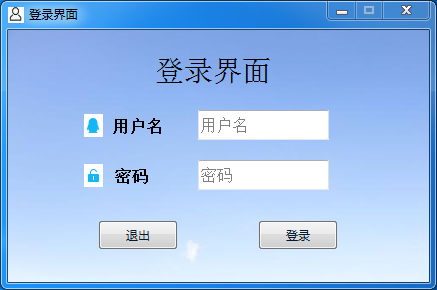
\includegraphics[width=0.6\textwidth]{登录.png}
	\caption[登录]{登录界面}\label{fig-login}
\end{figure}

%商品入库界面,在条形框中输入入库商品的基本信息后,点击入库实现商品成功入库,如图\ref{fig-save}
%\begin{figure}[H]
%	% 允许各个位置
%	\centering
%	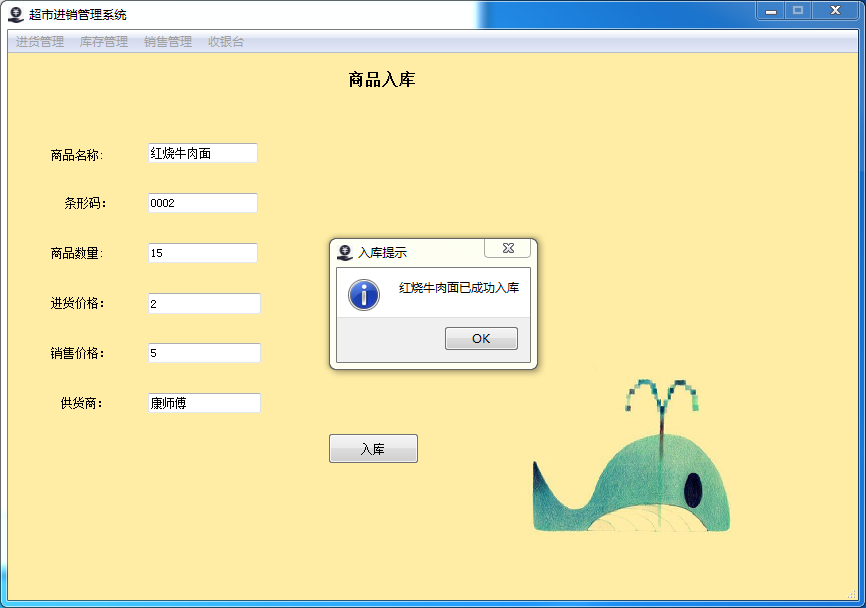
\includegraphics[width=0.8\textwidth]{商品入库.png}
%	\caption[商品入库]{商品入库}\label{fig-save}
%\end{figure}
库存浏览界面,点击查看库存便能显示所有库存商品信息,点击打印库存清单实现保存库存商品信息至指定目录。点击查找按钮,查询所有缺货商品。如图\ref{fig-show}
\begin{figure}[H]
	% 允许各个位置
	\centering
	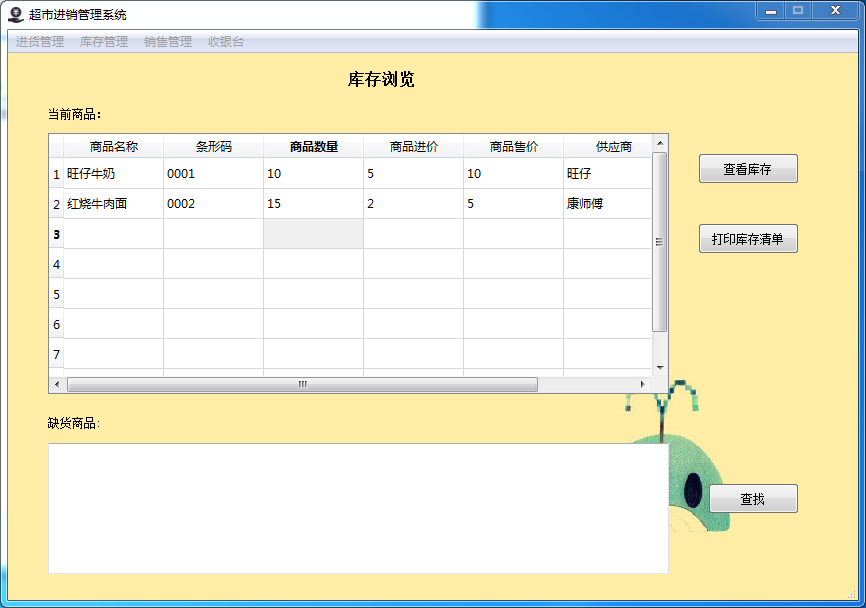
\includegraphics[width=0.7\textwidth]{库存查看.png}
	\caption[库存查看]{库存查看}\label{fig-show}
\end{figure}
信息修改界面,通过输入想要查找商品名称,查找到商品所有信息,对LineEdit修改后点击修改按钮进行商品信息修改,若想要删除商品则点击删除商品。如图\ref{fig-change}
\begin{figure}[H]
	% 允许各个位置
	\centering
	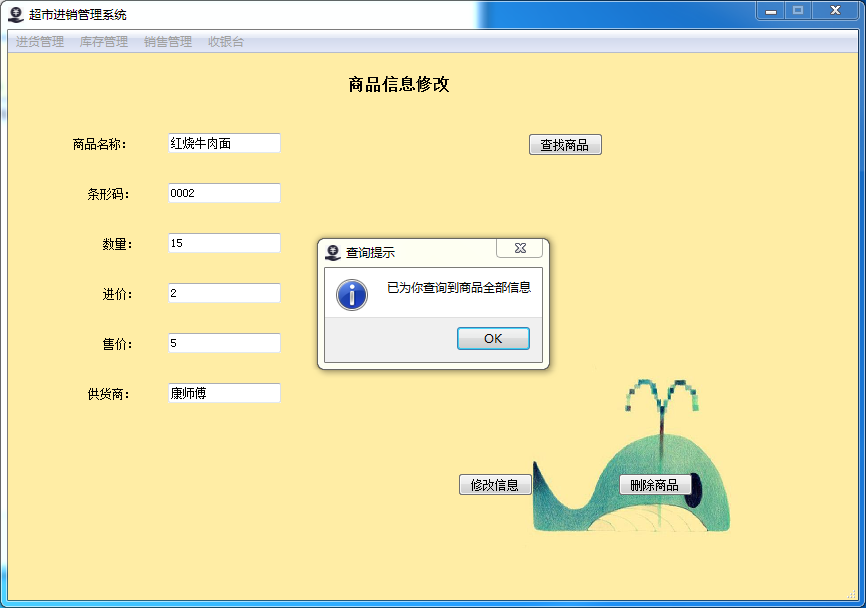
\includegraphics[width=0.7\textwidth]{信息修改.png}
	\caption[信息修改]{信息修改}\label{fig-change}
\end{figure}
%
%\begin{figure}[H]
%	% 允许各个位置
%	\centering
%	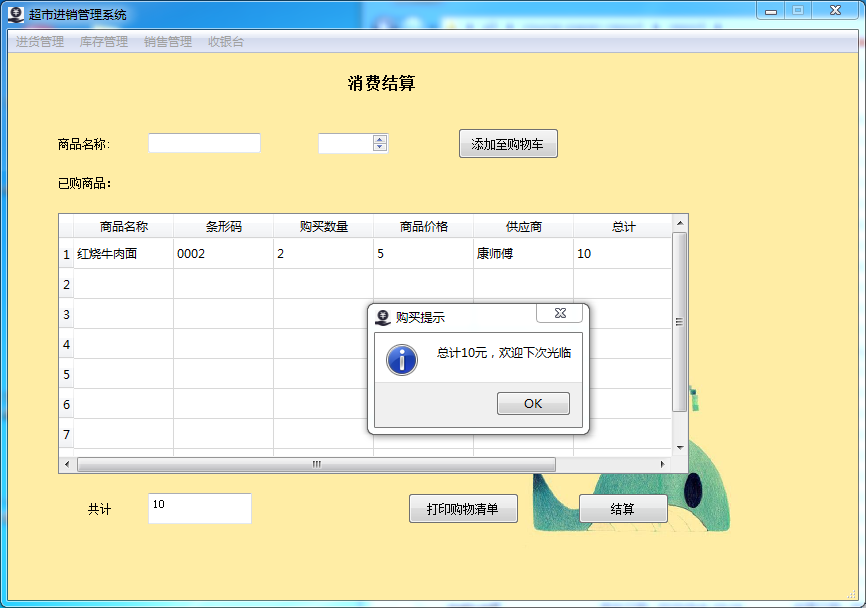
\includegraphics[width=0.8\textwidth]{购物结算.png}
%	\caption[购物结算]{购物结算}\label{fig-buy}
%\end{figure}
进入销售情况界面就能在TextEdit中查看到近期的商品进出库情况展示,点击打印销售清单便能成功保存打印。点击统计后便能查看当前商品的总营业额。如图\ref{fig-qingkuang}
\begin{figure}[H]
	% 允许各个位置
	\centering
	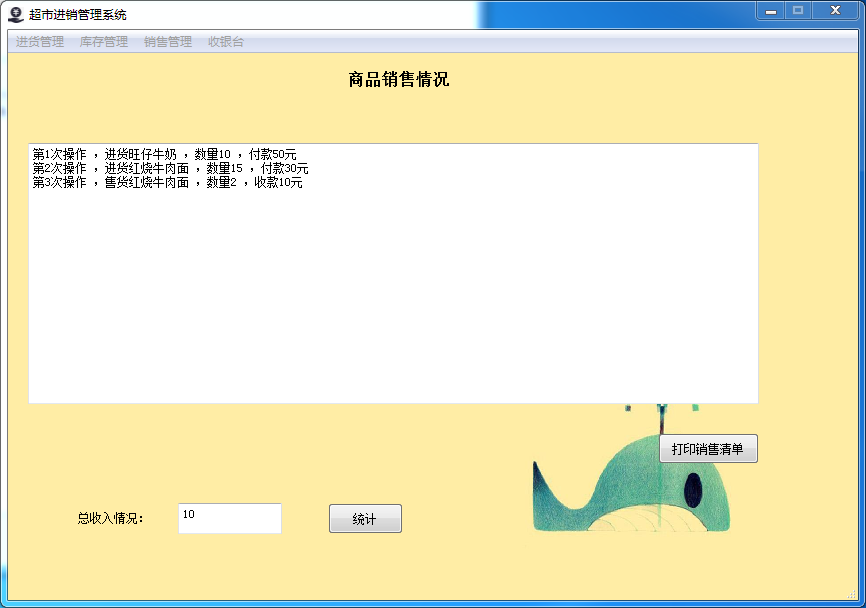
\includegraphics[width=0.7\textwidth]{销售情况.png}
	\caption[销售情况]{销售情况}\label{fig-qingkuang}
\end{figure}
\section{实习日志}
\subsection{8月24日}
主要任务:确定项目总体设计与模块划分

主要进行了如下工作:
\begin{enumerate}
	\item 需求分析,分析超市进销管理系统所需要的功能
	\item 对系统的界面进行一个大致的框架设计
	\item 所使用的工具进行确认,使用c++语言下的QT ,使用gitee代为管理代码,并用\LaTeX 代为编写实习报告.
	\item 类图的分析与设计
\end{enumerate}


我们选择的题目是超市进销管理系统,基于上学期期末选择的书店管理系统,我们这次选择这超市进销管理系统,准备在上次的基础上进行一些提高,让功能的实现更加立体化,并还原真正的超市管理系统。第一天我们选择不着急开始敲写代码,毕竟磨刀不误砍柴工,我们选择先开始对QT进行一些学习和了解,并在老师的指导下学习用git来完成分工协作,将自己的代码上传,更新远端的代码,将团队成员所做的贡献获取下来。最后我们进行了对我们管理系统类图的分析和设计。
\subsection{8月25日}
主要任务:完成类的设计以及界面的框架实现

主要进行了如下工作:
\begin{enumerate}
	\item 对类的基本分析以及类的设计和实现
	\item 继续对超市进销管理系统的功能和实现进行讨论并确定方案
	\item 设计和确定ui主界面,设计stacked widget的各个界面的总体框架布局规划
\end{enumerate}


今天我们就开始了正式的项目启动了,首要的是对商品类的设计,确定了商品的几大必要的基本属性以及成员函数,并予以实现。接着继续对系统的功能进行了讨论,最终确定了有进货管理,库存管理,销售管理,收银台,四个功能区域,并初步设计了使用stacked widget分开对每个模块进行设计,并完成两人的分工。

\subsection{8月26日}
主要任务:创建和完善用户登录界面

	今天的主要任务就是完成用户登录界面,在网络上搜索,有许多个版本的登录界面的设计方案,在其中进行有效的挑选后。第一次的选择出现错误,在信号与槽的发射方面还是不太精通,因此选择了一个更加有效和易懂的登录界面,参考还原真正的管理系统,我们创建了这样一个用户登录界面,并修改了其部分自带属性,来使其更加真实的模拟真实登录界面。
\subsection{8月27日}
主要任务:完成槽函数的设计(主要是对商品库存管理界面的功能实现)

	今天的主要任务是完成商品库存管理界面的实现,由于使用了QMap的STL 库,我边上网查找了许多关于c++的STL库中的map的资料进行学习,使用了QMap中的许多成员函数进行操作,结合队友完成的这个模块的ui界面进行连接操作,经过多方面的比对后,最后选择用QTableView这个组件来代替原本的文本框来盛放保存库存商品的信息,这样使得我们的系统在展示库存商品情况方面更加立体化和形象化。于是在下午又对QTableView进行研究,研究他的使用方法,参考网上的代码,理解了很长时间。虽然十分复杂,但是不断梳理还是明白了用QTableView 和QStandardItemModel 进行连接,用QStandardItemModel盛放数据,QTableView盛放表格的基本形式。
\subsection{8月28日}
主要任务:完成槽函数的设计(主要是对商品销售管理功能的设计和实现)

	今天的主要任务是完成销售管理系统界面的设计,经过讨论,将当日的流水清单进行展示还是需要在各个功能实现的情况下,进行新增,于是我在git上下载了队友的成果,并在进货管理和购物车的结算环节加入了一定的成员函数,使得当日的流水清单能够正常的打印。并设计了一个计算当日营业额的小函数插入其中。
	
	由于程序基本的框架已经浮现,我便进行了一次大整合,将我们两个所完成的部分的代码在git上进行比对和查看。完成整合后,我们对管理系统进行了小小的调试和讨论,对其中发现的一些小小的不合理的bug进行了修复,如进货名称不能为空,总计金额的LineEdit要设置为不可写入,等等。除此之外,我们也对下一步的代码编写做了一些总结,新增了一个文件处理功能由我来实现,一个ui界面的美化由队友来实现
\subsection{8月31日}
主要任务:完成文件处理的功能模块

今天最主要的任务是完成文件的处理功能,使我们的系统能够将库存商品信息,销售商品流水情况以及购物清单保存文件操作。
开始的时候使用的是QFile 以及文本输出流QTextStream 分别取库存商品信息,用户购物清单,以及超市进销库存流水信息的文本内容,放入out输出流中输出。可是由于这样的操作导致存放的文件的位置固定,无法特定保存,因此又上网查阅资料寻找了解决的方法,使用了QT中的的QFileDialog 类,用来完成选择文件夹,用类中的成员函数getSaveFileName实现调出设置
文件对话框。结果又出现了输出内容保存进文件后出现所有内容保存在一行之中,输出不了换行。经过长时间的检查和上网查问,发现win系统的回车符号有所不同。在修改后就完成了文件打印功能的实现。
\subsection{9月1日}
主要任务:程序的大测试以及课程报告的\LaTeX 初步编写

今天的任务就是对我们合作完成的超市进销管理系统 进行一次大复查,检查系统中不合理的,出现问题的部分。对产生问题的部分进行修改。对ui界面的背景等等进行调整。对一些临界点,极值点,进行测试和调试,保证代码程序不会出现漏洞bug。

与此同时,展开对课程实习报告的\LaTeX 编写,让自己重新梳理对这个系统的框架,整理出框架便于自己有条不紊的完成对课程论文报告中自己完成的部分进行写作
\subsection{9月2日}
主要任务:程序的借鉴以及可测和那个报告的正式编写

今天的任务是借鉴网络上和同学们程序代码中用的好的部分进行学习和借鉴,丰富自己的代码,和一些小小的贴心的小细节。

同时正式开始对课程报告进行书写,完成论文的大部分自己负责的部分,并开始对自己这两周的实习进行总结和阐述。
\subsection{9月3日}
主要任务:准备答辩PPT,以及准备答辩的内容

今天,针对所完成的超市进销管理系统进行重新回顾,和队友确认负责部分以及分别讲对这次实习所完成部分的细节。接下来就是对自己答辩部分进行熟悉,确定自己答辩的方向

\subsection{9月4日}
主要任务:进行实习答辩,继续完善论文部分

今天开始完成答辩,向老师介绍自己的项目以及自己所负责的部分的实现。和老师进行良好的沟通,老师也给我们提供了许多改进的思路和方法,并分析了我们目前出现的错误和原因,为我们未来完善这个软件提供了帮助。

\section{实习总结}
本次为期两个星期的实习是我感触比较深的实习,由于春季学期正值疫情,我们在家中完成了面向对象程序设计这门课程的学习,由于在家中学习,并没有很高的学习效率。因此\ccpp 编程水平仍有欠缺,在上学期结课时选择了书店管理系统,勉勉强强完成了管理系统的设计。这次夏季学期选择的超市进销管理系统,相比于书店管理系统,类的成分会减少些许,但是在功能方面却有所增加。我和我的队友,在上学期的书店管理系统设计的背景下,学习了我当时运用的较好的Qmap 键值对用来保存商品信息,方便数据的遍历。也总结了当时书店管理系统所存在的问题,在长达两个星期的调试中,一次一次的改进代码,优化程序,清除bug.

还有与上次大作业不同的是,这次我们采取了两人合作的形式完成超市进销管理系统的设计。虽然说人多力量大,但是在两个的协调分工合作方面,我们也确实产生了一点问题。由于不停的产生代码的修改,两个人的代码更新就较为困难。在老师的建议下,我们选择使用了gitee这个平台进行协作合同,并早在实习前将其弄懂。每个人通过pull,fetch 等等操作将自己的代码上传,更新远端的代码,用这个平台管理我们自己的代码。我也负责在其中将两人的代码进行整合管理。

对于QT这个\ccpp 用户开发框架,刚上手是确实不适应。在一段时间熟悉后,我们发现,Qt中信号与槽,是他脱颖而出的最大关键,通过这个特性,我们可以实现一系列的连接操作。除此之外,Qt中部分内置的类也有许多强大的功能,通过使用这些类或者继承这些类,然后完成我们自己类的设定,方便了我们程序的开发以及设计。

在这两周的实习过程中,必然的,我们也遇到了许多问题。如何掌握一个全新不认识的类,通过向学长,向同学,老师请教,我逐渐开始明白了怎么剖析一个类,查询它的父类子类,查询它的共有属性和专属的特殊属性,函数,信号槽。通过这次实习中,我们所克服的这些困难,我们也积累了许多的经验,我收获了许多,不仅仅是知识层面上的,比如说本次实习在代码上采用的是Qt设计,报告上采用的是\LaTeX ,在代码管理方面采用的是Git。更多的是一种经验,让自己知道,再大的困难也能克服。

虽然本次实习选择的课题难度并不是很大,但是我认为,能把简单的程序做到最优化,做到最精致,不停地反复调试,难道不应该也是一件有挑战的任务吗?只有不断反问自己,还能更优化代码了吗?
还能再新增功能了吗?做到精益求精,我认为未尝不是一个挑战。
\section{附录:核心代码清单}
本项目的代码上传至Gitee网站管理,项目地址:https://gitee.com/CH3OCH3/c-internship

接下来展示负责部分的核心代码。

由于部分代码已在上文介绍功能实现中展示,不做过多赘述如代码清单\ref{code1}\ref{code2}\ref{code3}\ref{code4}\ref{code5}\ref{code6}\ref{code7}\ref{code8}
\begin{langCVOne}[C++][code9][QT]{login.h/login.cpp}
login.h
#ifndef LOGIN_H
#define LOGIN_H

#include <QWidget>

namespace Ui {
    class login;
}

class login : public QWidget
{
    Q_OBJECT	
    public:
    explicit login(QWidget *parent = nullptr);
    ~login();
    void paintEvent(QPaintEvent *);
    private slots:
    void on_pushButton_2_clicked();
    void on_pushButton_clicked();
    private:
    Ui::login *ui;
};
#endif // LOGIN_H


login.cpp
#include "login.h"
#include "ui_login.h"
#include "mainwindow.h"
#include <QMessageBox>
#include<QPainter>
login::login(QWidget *parent) :
QWidget(parent),
ui(new Ui::login)
{
    ui->setupUi(this);
}

login::~login()
{
    delete ui;
}

void login::on_pushButton_2_clicked()
{
    this->close();
}

void login::on_pushButton_clicked()
{
    QString username = ui->useredit->text();
    QString password = ui->passedit->text();
    if(username=="admin" && password=="123456")
    {
        QMessageBox::information(this,"登录提示","登录成功");
        this->close();
        MainWindow * t=new MainWindow;
        t->setWindowTitle("超市进销管理系统");
        t->setFixedSize(850,570);
        t->setWindowIcon(QIcon(":/photo/shop.jpg"));
        t->show();
    }
    else
    {
        QMessageBox::information(this,"登录提示","用户名或密码错误");
        ui->useredit->clear();
        ui->passedit->clear();
    }
}
void login:: paintEvent(QPaintEvent *)
{
    QPainter painter(this);
    QPixmap pix;
    pix.load(":/photo/u=2413354430,3009708332&fm=26&gp=0.jpg");
    painter.drawPixmap(0,0,this->width(),this->height(),pix);
    //  画背景上图标
    //  pix.load(":/photo/ziti.jpg_w800");
    //  缩放
    //  pix = pix.scaled(pix.width()*0.5,pix.height()*0.5);
    //  painter.drawPixmap(10,30,pix);
}
\end{langCVOne}
此处放出MainWindow.h/MainWindow.cpp中部分未展示代码
\begin{langCVOne}[C++][code10][QT]{MainWindow.h/MainWindow.cpp}
MainWindow.h
#ifndef MAINWINDOW_H
#define MAINWINDOW_H

#include <QMainWindow>
#include <QMap>
#include <good.h>
#include <QMessageBox>
#include <QSpinBox>
#include <QDebug>
#include <QFile>
#include <QFileDialog>
#include<QPainter>
#include <QTableView>
#include <QListView>
#include <QTreeWidget>
#include <QStandardItemModel>
#include <QStandardItem>
QT_BEGIN_NAMESPACE
namespace Ui { class MainWindow; }
QT_END_NAMESPACE

class MainWindow : public QMainWindow
{
    Q_OBJECT
    
    public:
    MainWindow(QWidget *parent = nullptr);
    ~MainWindow();
    void paintEvent(QPaintEvent *);
    QTableView * table_view;
    QStandardItemModel * item_model;
    QTableView * table_view_2;
    QStandardItemModel * item_model_2;
    void inittable();
    private:
    Ui::MainWindow *ui;
    QMap<QString ,Good *> shop;
    QMap<QString ,Good *> car;
    private slots:
    void in_();
    void stock_();
    void income_();
    void sale_();
    void change_();
    void on_input_clicked();
    void on_findbtn_clicked();
    void on_pushButton_clicked();
    void on_incar_clicked();
    void on_paytotal_clicked();
    void on_findbtn_2_clicked();
    void on_changebtn_clicked();
    void on_deletebtn_clicked();
    void on_totalbtn_clicked();
    void on_printbtn_clicked();
    void on_printbtn_2_clicked();
    void on_printbtn_3_clicked();
};

MainWindow.cpp
#include "mainwindow.h"
#include "ui_mainwindow.h"
#include <QMessageBox>
#include <QSpinBox>
#include <QDebug>
#include <QFile>
#include <QFileDialog>
#include<QPainter>
#include <QTableView>
#include <QListView>
#include <QTreeWidget>
#include <QStandardItemModel>
#include <QStandardItem>
QString water;
int count=1;
double money=0;

MainWindow::MainWindow(QWidget *parent)
: QMainWindow(parent)
, ui(new Ui::MainWindow)
{
    ui->setupUi(this);
    connect(ui->incontrol,&QMenu::triggered,this,&MainWindow::in_);
    connect(ui->stock,&QAction::triggered,this,&MainWindow::stock_);
    connect(ui->incomecontrol,&QMenu::triggered,this,&MainWindow::income_);
    connect(ui->salecontrol,&QMenu::triggered,this,&MainWindow::sale_);
    connect(ui->change,&QAction::triggered,this,&MainWindow::change_);
    inittable();
}

MainWindow::~MainWindow()
{
    delete ui;
}
void MainWindow::inittable()
{
    table_view = ui->tableView;
    item_model = new QStandardItemModel(8,4);  // 4行4列
    table_view->setModel(item_model);//两者关联
    QStringList column, row;//行列表头
    column << "商品名称" << "条形码" << "商品数量" << "商品进价" << "商品售价"  << "供应商" ;
    row << "1" << "2" << "3" << "4";
    item_model->setHorizontalHeaderLabels(column);                // 设置水平表头标签
    item_model->setVerticalHeaderLabels(row);
    table_view->setEditTriggers(QTreeView::NoEditTriggers);
    
    
    table_view_2 = ui->tableView_2;
    item_model_2 = new QStandardItemModel(8,4);  // 4行4列
    table_view_2->setModel(item_model_2);//两者关联
    QStringList column2, row2;//行列表头
    column2 << "商品名称" << "条形码" << "购买数量"  << "商品价格"  << "供应商" << "总计";
    row2 << "1" << "2" << "3" << "4";
    item_model_2->setHorizontalHeaderLabels(column2);                // 设置水平表头标签
    item_model_2->setVerticalHeaderLabels(row2);
    table_view_2->setEditTriggers(QTreeView::NoEditTriggers);
}
void MainWindow::on_findbtn_clicked()
{
    QString list;
    int s=0;
    QMap<QString ,Good*>::Iterator it;
    for(it=shop.begin();it!=shop.end();it++)
    {
        QString str ;
        if(it.value()->getnumber()==0)
        {          
            str =QString("%1已经缺货,请及时补货").arg(it.value()->getname());
            str=str+"\n";
            s++;
        }
        list=list+str;
    }
    if(s==0) QMessageBox::information(this,"提示","库存中未存在缺货商品");
    else QMessageBox::information(this,"提示","以为你展示全部缺货商品");
    
    ui->textEdit->setText(list);
}
void MainWindow::on_pushButton_clicked()
{
    item_model->clear();
    item_model = new QStandardItemModel(8,4);  // 4行4列
    table_view->setModel(item_model);//两者关联
    //table_view->setSortingEnabled(true);
    QStringList column, row;//行列表头
    column << "商品名称" << "条形码" << "商品数量" << "商品进价" << "商品售价"  << "供应商" ;
    row << "1" << "2" << "3" << "4";
    item_model->setHorizontalHeaderLabels(column);                // 设置水平表头标签
    item_model->setVerticalHeaderLabels(row);
    table_view->setEditTriggers(QTreeView::NoEditTriggers);
    
    QMap<QString ,Good*>::Iterator itt;
    int i=0;
    for(itt=shop.begin();itt!=shop.end();itt++)
    {
        item_model->setItem(i,0,new QStandardItem(QString("%1").arg(itt.value()->getname())));
        item_model->setItem(i,1,new QStandardItem(QString("%1").arg(itt.value()->getcode())));
        item_model->setItem(i,2,new QStandardItem(QString("%1").arg(itt.value()->getnumber())));
        item_model->setItem(i,3,new QStandardItem(QString("%1").arg(itt.value()->getinprice())));
        item_model->setItem(i,4,new QStandardItem(QString("%1").arg(itt.value()->getoutprice())));
        item_model->setItem(i,5,new QStandardItem(QString("%1").arg(itt.value()->getsupplier())));
        i++;
    }
    QMessageBox::information(this,"提示","已为你显示全部库存信息");
    QString list;
    QMap<QString ,Good*>::Iterator it;
    for(it=shop.begin();it!=shop.end();it++)
    {
        QString str;
        str=QString("商品名称:%1  条形码:%2  数量:%3  进价:%4  售价:%5  供应商:%6").arg(it.value()->getname()).arg(it.value()->getcode()).arg(it.value()->getnumber()).arg(it.value()->getinprice()).arg(it.value()->getoutprice()).arg(it.value()->getsupplier());
        str=str+"\n";
        list=list+str;
    }
    ui->information->setText(list);
}
void MainWindow:: paintEvent(QPaintEvent *)
{
    QPainter painter(this);
    QPixmap pix;
    pix.load(":/photo/timg.jpg");
    painter.drawPixmap(0,0,this->width(),this->height(),pix);
    
    //  画背景上图标
    //  pix.load(":/photo/ziti.jpg_w800");
    //  缩放
    //  pix = pix.scaled(pix.width()*0.5,pix.height()*0.5);
    //  painter.drawPixmap(10,30,pix);
}
\end{langCVOne}
\end{document}

%%% Local Variables:
%%% mode: latex
%%% TeX-master: t
%%% End:
